\section{Tangentes}

La pente est calculée par Lua dans les unités du repère : une tangente est donc correcte même si \tkzname{xstep} et \tkzname{ystep} sont différents. Chaque tangente est formée de deux demi-tangentes : à gauche (l = left) et à droite (r = right). Leurs longueurs sont données par \tkzname{kl} et \tkzname{kr}, en unités de l'axe des abscisses : la demi-tangente à droite va du point de contact $(a~;~f(a))$ au point $(a+k_r~;~f(a)+k_r f'_d(a))$. Avec $kl=0$ ou $kr=0$, la demi-tangente correspondante n'est pas tracée.

Si la fonction n'est pas dérivable en $a$, les deux demi-tangentes ont des pentes différentes ; elles sont calculées séparément.

\subsection{Représentation d'une tangente : \tkzcname{tkzFnTangent}}

\begin{NewMacroBox}{tkzFnTangent}{\oarg{options}\parg{nom de la fonction,$a$}}
\begin{tabular}{lll}
 \toprule
 arguments             & exemple & explication    \\
 \midrule
 \TAline{fonction,a}{(f,0)}{tangente au point d'abscisse $0$}
 \bottomrule
\end{tabular}

\begin{tabular}{lll}
\toprule
options             & défaut & définition                         \\
\midrule
\TOline{draw}{false}{le point de contact est tracé}
\TOline{kl}{1}{longueur de la demi-tangente à gauche (unités de l'axe des abscisses)}
\TOline{kr}{1}{longueur de la demi-tangente à droite}
\TOline{clip}{true}{la tangente est découpée à la fenêtre}
\bottomrule
\end{tabular}

\emph{Les autres options sont celles de \TIKZ ; le style est \tkzname{tkzfn tangent}, vide par défaut. Pour retrouver les flèches de \tkzname{tkz-fct} :}

|\tikzset{tkzfn tangent/.style={->,>=latex}}|
\end{NewMacroBox}

\tkzHand La fonction n'a pas besoin d'être tracée, il suffit qu'elle soit définie.

%<--------------------------------------------------------------------------->
\subsection{Tangente avec \tkzname{xstep} et \tkzname{ystep} différents de 1}

Il n'est pas nécessaire de faire des calculs : il suffit d'utiliser les valeurs qui correspondent aux graduations.

\begin{tkzexample}[vbox]
\begin{tikzpicture}[xscale=1.5]
 \tkzFnInit[xmin=0,xmax=800,xstep=100,
            ymin=0,ymax=1800,ystep=400]
 \tkzFnGrid[color=brown,sub,subdx=50,subdy=200](0,0)(800,1800)
 \tkzFnAxes
 \tkzFnDraw[name=f,color=red,samples=100,domain=0:800]
    {(1/90000)*x^3-(1/100)*x^2+(113/36)*x}
 \tkzFnTangent[draw,color=blue,kr=300,kl=450](f,450)
 \tkzFnText[draw,color=black,fill=brown!50,opacity=0.8](300,1200)
 {$f(x)=\dfrac{1}{90000}x^3 -\dfrac{1}{{100}}x^2 +\dfrac{113}{36}x$}
\end{tikzpicture}
\end{tkzexample}

La pente en $450$ est $\tkzFnPrint[4]{diff(f,450)}$ ; on l'obtient avec |\tkzFnPrint[4]{diff(f,450)}|.

%<--------------------------------------------------------------------------->
\subsection{Les options \tkzname{kl}, \tkzname{kr} et l'option \tkzname{draw}}

\begin{tkzexample}[]
\begin{tikzpicture}[scale=1.5]
  \tikzset{tkzfn tangent/.style={->,>=latex}}
  \tkzFnInit[xmin=-3,xmax=4,ymin=-4,ymax=2]
  \tkzFnGrid  \tkzFnAxes[ticks=false]
  \tkzFnDraw[name=f,domain=-2.15:3.2]{-x*x+2*x}
  \tkzFnDefPoint[draw](f,2){A}
  \tkzFnTangent[kl=0,draw](f,-1)
  \tkzFnTangent[draw](f,1)
  \tkzFnTangent[kr=0,draw](f,3)
  \tkzFnRep
\end{tikzpicture}
\end{tkzexample}

%<--------------------------------------------------------------------------->
\subsection{Tangente et deux fonctions}
L'option \tkzname{with} de \tkzname{tkz-fct} n'existe plus : la fonction est désignée par son nom.

\begin{tkzexample}[]
\begin{tikzpicture}[scale=4]
 \tkzFnInit[xmin=0,xmax=3,ymin=0,ymax=2]
 \tkzFnAxes
 \tkzFnGrid(0,0)(3,2)
 \tkzFnDraw[name=f,color=red,domain=1/3:3]
           {0.125*(3*x-1)+0.375*(3*x-1)/(x*x)}
 \tkzFnDraw[name=g,color=blue,domain=1/3:3]
           {0.125*(3*x-1)}
 \tkzFnTangent[color=blue](f,1)
 \tkzFnText[draw,color=red](1,1.5)
   {$f(x)=\frac{1}{8}(3x-1)+\frac{3}{8}\left(\frac{3x-1}{x^2}\right)$}
 \tkzFnText[draw,color=blue](2,0.3)
   {$g(x)=\frac{1}{8}(3x-1)$}
\end{tikzpicture}
\end{tkzexample}

%<--------------------------------------------------------------------------->
\subsection{Quelques tangentes}

\begin{tkzexample}[]
\begin{tikzpicture}[scale=2]
  \tkzFnInit[xmin=-5,xmax=2,ymin=-1,ymax=3]
  \tkzFnAxes[ticks=false]
  \tkzFnText[draw,color=red,fill=orange!20](1.5,1.5){$y = xe^x$}
  \tkzFnDraw[name=f,color=red,domain=-5:1]{x*exp(x)}
  \tkzFnTangent[color=blue,kr=2,kl=2](f,-2)
  \tkzFnTangent[color=green,kr=2,kl=2](f,-1)
  \tkzFnTangent[color=blue](f,0)
  \tkzFnTangent[color=blue,kr=0](f,1)
\end{tikzpicture}
\end{tkzexample}

%<--------------------------------------------------------------------------->
\subsection{Demi-tangentes}
En $0$, la fonction $f$ définie par $f(x)=\sqrt{x^3+x^2}$ n'est pas dérivable : les deux demi-tangentes sont obtenues automatiquement.

\begin{tkzexample}[]
 \begin{tikzpicture}[scale=2.75]
     \tkzFnInit[xmin=-2,xmax=3,ymin=0,ymax=3]
     \tkzFnGrid[color=orange](-2,0)(3,3)
     \tkzFnAxes
     \tkzFnDraw[name=f,color=red,domain=-1:2]{sqrt(x^3+x^2)}
     \tkzFnTangent(f,0)
     \tkzFnText[draw,color=red,fill=orange!20](2,1){$f(x)=\sqrt{x^3+x^2}$}
 \end{tikzpicture}
\end{tkzexample}

%<--------------------------------------------------------------------------->
\subsection{Demi-tangentes : courbe de Lorentz}

Ici, on ne veut que les demi-tangentes comprises entre 0 et 1 : il suffit de donner la valeur 0 à \tkzname{kl} dans un cas et à \tkzname{kr} dans l'autre.

\begin{center}
\begin{tkzexample}[vbox]
\begin{tikzpicture}[scale=1.25]
  \tkzFnInit[xmin=0,xmax=1,ymin=0,ymax=1,xstep=0.1,ystep=0.1]
  \tkzFnGrid(0,0)(1,1)
  \tkzFnAxes
  \tkzFnDraw[name=f,color=red,thick,domain=0:1]{(exp(x)-1)/(exp(1)-1)}
  \tkzFnTangent[draw,kl=0,  kr=0.4](f,0)
  \tkzFnTangent[draw,kl=0.4,kr=0  ](f,1)
  \tkzFnText[draw,color=red,fill=orange!20](0.5,0.6)
          {$f(x)=\dfrac{\text{e}^x-1}{\text{e}-1}$}
\end{tikzpicture}
\end{tkzexample}
\end{center}

%<--------------------------------------------------------------------------->
\subsection{Série de tangentes}

Les tangentes peuvent être tracées dans une boucle \tkzcname{foreach}.

\begin{tkzexample}[vbox]
\begin{tikzpicture}[scale=2]
  \tkzFnInit[xmin=-5,xmax=2,ymin=-1,ymax=3]
  \tkzFnAxes[ticks=false]
  \tkzFnText[draw,color=red,fill=orange!20](1.5,1.5){$y = xe^x$}
  \tkzFnDraw[name=f,line width=0.01pt,color=red,domain=-5:1]{x*exp(x)}
  \foreach \v in {-4,-3.8,...,0}{
    \tkzFnTangent[color=blue,line width=.4pt,kr=1,kl=0.5](f,\v)}
  \foreach \v in {0.6,0.8,1}{
    \tkzFnTangent[color=blue,line width=.4pt,kr=0,kl=0.5](f,\v)}
\end{tikzpicture}
\end{tkzexample}

%<--------------------------------------------------------------------------->
\subsection{Série de tangentes sans courbe}

La fonction est définie par \tkzcname{tkzFnDef} mais n'est pas tracée.

\begin{tkzexample}[vbox]
\begin{tikzpicture}[scale=2]
  \tkzFnInit[xmin=-5,xmax=2,ymin=-1,ymax=3]
  \tkzFnAxes[ticks=false]
  \tkzFnText[draw,color=red,fill=orange!20](1.5,1.5){$y = xe^x$}
  \tkzFnDef{f}{x*exp(x)}
  \foreach \v in {-4,-3.8,...,0}{
    \tkzFnTangent[color=blue,line width=.4pt,kl=1](f,\v)}
  \foreach \v in {0.6,0.8,1}{
    \tkzFnTangent[color=blue,line width=.4pt,kr=0,kl=.75](f,\v)}
\end{tikzpicture}
\end{tkzexample}

\newpage
\subsection{Abscisse donnée par une expression}

L'abscisse du point de contact peut être une expression Lua ; si elle contient des parenthèses, on la place entre accolades.

\begin{center}
\begin{tkzexample}[]
\begin{tikzpicture}[scale=1]
  \tkzFnInit[xmin=0,xmax=1,xstep=0.1,
             ymin=0.5,ymax=1,ystep=0.1]
  \tkzFnGrid \tkzFnAxes
  \tkzFnDraw[name=f,domain=0.00001:1]{x^x}
  \tkzFnTangent[draw,color=red,kr=0.2,kl=0.2](f,{1/exp(1)})
\end{tikzpicture}
\end{tkzexample}
\end{center}

\endinput
